\section{Correlated Subgraph Search Tree}
\label{sec:searchTree}
In this section, we depict the detailed structure of the search tree. All the operations including subgraph extension, correlation calculation, and further analysis are based on this correlated subgraph search tree.


% Firstly, we denote two events for better expression.

% \squishlist
% \item{\sf Found($Q$).} denotes the event that subgraph $Q$ is discovered and checked as a frequent subgraph, in a word, $Q$ is found.
% \squishend
% \squishlist
% \item{\sf Op($Q$).} denotes the event that the we calculate the correlation of $Q$ and extend $Q$, in a word, $Q$ is operated.
% \squishend

We denote the search tree as $T$, each node $Q,Q\in T$ represents a subgraph pattern. We denote the set of current leaf nodes in the search tree as $Leaf(T)$, each element $Q_l$, where $Q_l\in Leaf(T)$, is a subgraph which has not yet been $operated$ for correlation computation. All the leaf nodes $Q_l\in Leaf(T)$, once operated are put into the set $operated$.
\subsection{Order of Subgraph Generation and Correlation Calculation}

\par Basically, our whole process is compounded by a series of loops, each of which contains 4 steps:
\par 1) select a node $Q_i$ from $Leaf(T)$, i.e. $Q_i\in Leaf(T)$, and pop out $Q_i$ from $Leaf(T)$, i.e. $Leaf(T)=Leaf(T)\setminus Q_i$.
\par 2) calculate $\tau(Q_i,Q_j,h)$, for all $Q_j\in operated$
\par 3) try to extend $Q_i$ to $Ex(Q_i)$, where $Ex(Q_i)$ is the set of all the possible subgraphs extended from $Q_i$.
\par 4) Check the frequency of $Q_i',Q_i'\in Ex(Q_i)$ based on MNI support, $\sigma(Q')$, if $\sigma(Q_i')\ge$ {\sf Min-Sup}. we put $Q_i'$ into $Leaf(T)$.
	\begin{thrm}
		The order of subgraph generation and correlation calculation will not miss any correlated pairs between any of two frequent subgraphs.
	\end{thrm}	
% After step 4, we give $Q_i'$ an index of frequent subgraph discovery order, denoted as $index(Q_i')=a$, which means $Q_i'$ is the $a$-th subgraph in $T$. After the loop, we give $Q_i$ an index of correlation calculation order, denoted as $corIndex(Q_i)=b$, which means $Q_i$ is the $b$-th subgraph in $T$ which and we put $Q_i$ into $Cor(T)$, i.e. $Cor(T)=Cor(T)\cap Q_i$.
\subsection{Best-first Search Strategy}
\subsubsection{Estimating Criteria}\label{subsubsec:estimating}
Observation \ref{ob:frequency} draws us a hint that we may reach our destination more quickly if we firstly extend the subgraphs which have the higher support. As a result, we use a naive rule to determine the priority of the leaf nodes, $Q_1$ has a higher priority than $Q_2$ if and only if:
	\begin{align*}\sigma(Q_1)>\sigma(Q_2)\end{align*}
Utilizing the estimating rule which is mentioned above, if the current leaf node $Q_k$ in the search tree has a highest support among all the other elements in the set of the leaf nodes, i.e. $\sigma(Q_k)=\max\{\sigma(Q_i)|Q_i\in Leaf(T)\}$. Then, $Q_k$ has the priorty to be calculated and extended.

\subsubsection{Ceasing mechanism}\label{subsubsec:ceasing}
Obviously, our purpose is to find $k$ pairs of correlated subgraphs and guarantee that the other pair of subgraphs could not have a higher correlation $\tau$. Retrospect the properties mentioned in Section \ref{sec:overview}, assume $Q$ is a frequent subgraph of the data graph, $Q_k$ is an arbitary frequent subgraph of the data graph. We denote $Sup(Q)$ as the set of all the possible supergraphs of $Q$ and $Q'\in Sup(Q)$. Then, the following condition always holds:
	\begin{align*} \tau(Q',Q_k,h)\le \sigma(Q') \end{align*}
	\begin{align*} \sigma(Q')\le \sigma(Q) \end{align*}
	It is easy to get following upperbound of $\tau(Q',Q_k,h)$ by combining the two conditions above:
	\begin{align*} \tau(Q',Q_k,h) \le \sigma(Q) \end{align*}
Consider this upperbound, if $\sigma(Q)$ does not reach the minimum number of being a candidate of {\sf Top-$k$} set, i.e. $\sigma(Q)<\tau(Q_i,Q_j,h)$ for all the $i, j$ in the current {\sf Top-$k$} set, then all the correlations containing $Q$, $\tau(Q,Q_k,h)$, as well as all the correlations containing $Q'$, $\tau(Q',Q_k,h)$, are impossible to be the elements in {\sf Top-$k$} set. 
\par On the other hand, we have to consider another possible circumstance, where there are no $k$ correlated pairs in this graph at all. In that case, the number of elements in {\sf Top-$k$} set has not reached $k$ but all the support value of the leaf nodes are already below the minimum support. As a consequence, this condition is also a signal telling us to stop the search.
\par Formally, we fix the condition of not adding $Q$ to $Leaf(T)$, which is, suppose $|Topk|$ is the number of elements in {\sf Top-$k$} set, $min\_sup$ is the minimum support of the correlation, we stop our search if either both of the following conditions holds.
\begin{align*} \sigma(Q)\le min\{t|t\in Top\_k\}\end{align*}
\begin{align*} |Top\_k|=k \end{align*}
or following condition holds.
\begin{align*} \sigma(Q)\le min\_sup\end{align*}
In this case, all the $Q,Q\in Leaf(T)$ is possible to have the correlation we want. Obviously, on the other hand, if $Leaf(T)=\emptyset$, we report all the {\sf Top-$k$} correlated subgraphs and cease our search.
\begin{figure}[t!]
\centering
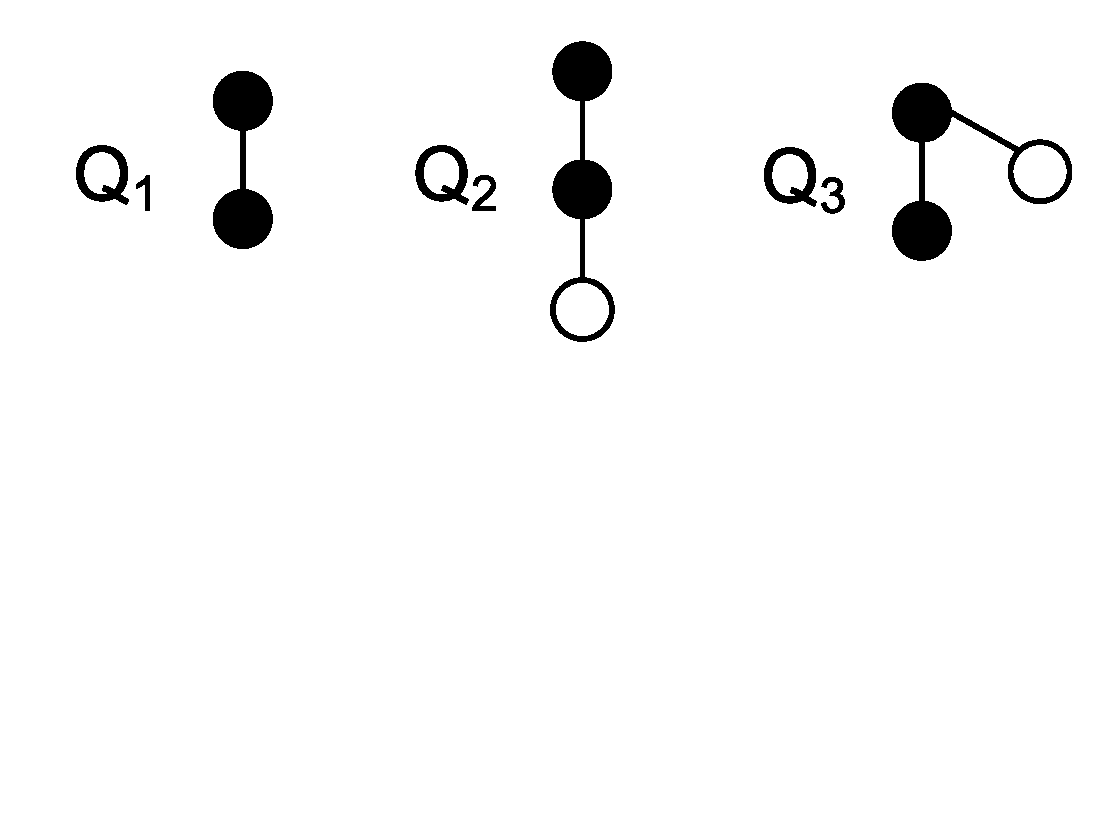
\includegraphics[scale=0.32]{images/ceasing_condition}
\vspace{-2mm}
\caption{\scriptsize For 3 subgraphs $Q_1,Q_2,Q_3$, with $\sigma(Q_1)=5$, $\sigma(Q_2)=2$, $\sigma(Q_3)=3$. The current {\sf Top-$k$} set is $\{4,5,6\}$, the input parameters are $k=3$, {\sf Min-sup}$=3$}.
\label{fig:ceasing_condition}
\vspace{-6mm}
\end{figure}
\begin{exple}
	In Figure \ref{fig:ceasing_condition}, the minimum element in {\sf Top-$k$} set is $4$, $Q_1$ is the only leaf node at the beginning, i.e. $Leaf(T)=\{Q_1\}$ and $\sigma(Q_1)>4$ so that $Q_1$ can be extended to $Q_2,Q_3$. After extension, $Q_1\notin Leaf(T)$ and $Leaf(T)=\{Q_2,Q_3\}$. $Q_2<$ {\sf Min-sup}, and $Q_3=$ {\sf Min-sup} but $Q_3<4$, and there are already $3$ elements in {\sf Top-$k$} set, i.e. $|Top\_k|=3$. Thus, all the correlation of $Q_2,Q_3$ would not satisfies the condition we want and we cease the search.
\end{exple}
\subsection{Search Tree Storage Unit}\label{subsec:unit}
Considering the large amount of overlaps of the instances in dense graph, we use a novel structure to store a subgraph pattern, which not only get rid of the expensive cost of tackling dense graph, but also be the robust foundation of carrying out an efficient correlation calculation based on instance grouping.
\par Our search tree storage unit is extremely direct and naive. Instead of considering the instances of a pattern, we just create a reproduce of the occurrences of the vertices and the edges of the pattern, called {\bf replica}. We record all the vertex identifications and the edge connections in the replica, we do not record the edge labels.
\begin{figure}[h!]
\vspace{-2mm}
\centering
\subfigure[{\scriptsize Subgraph Pattern $Q$}] {
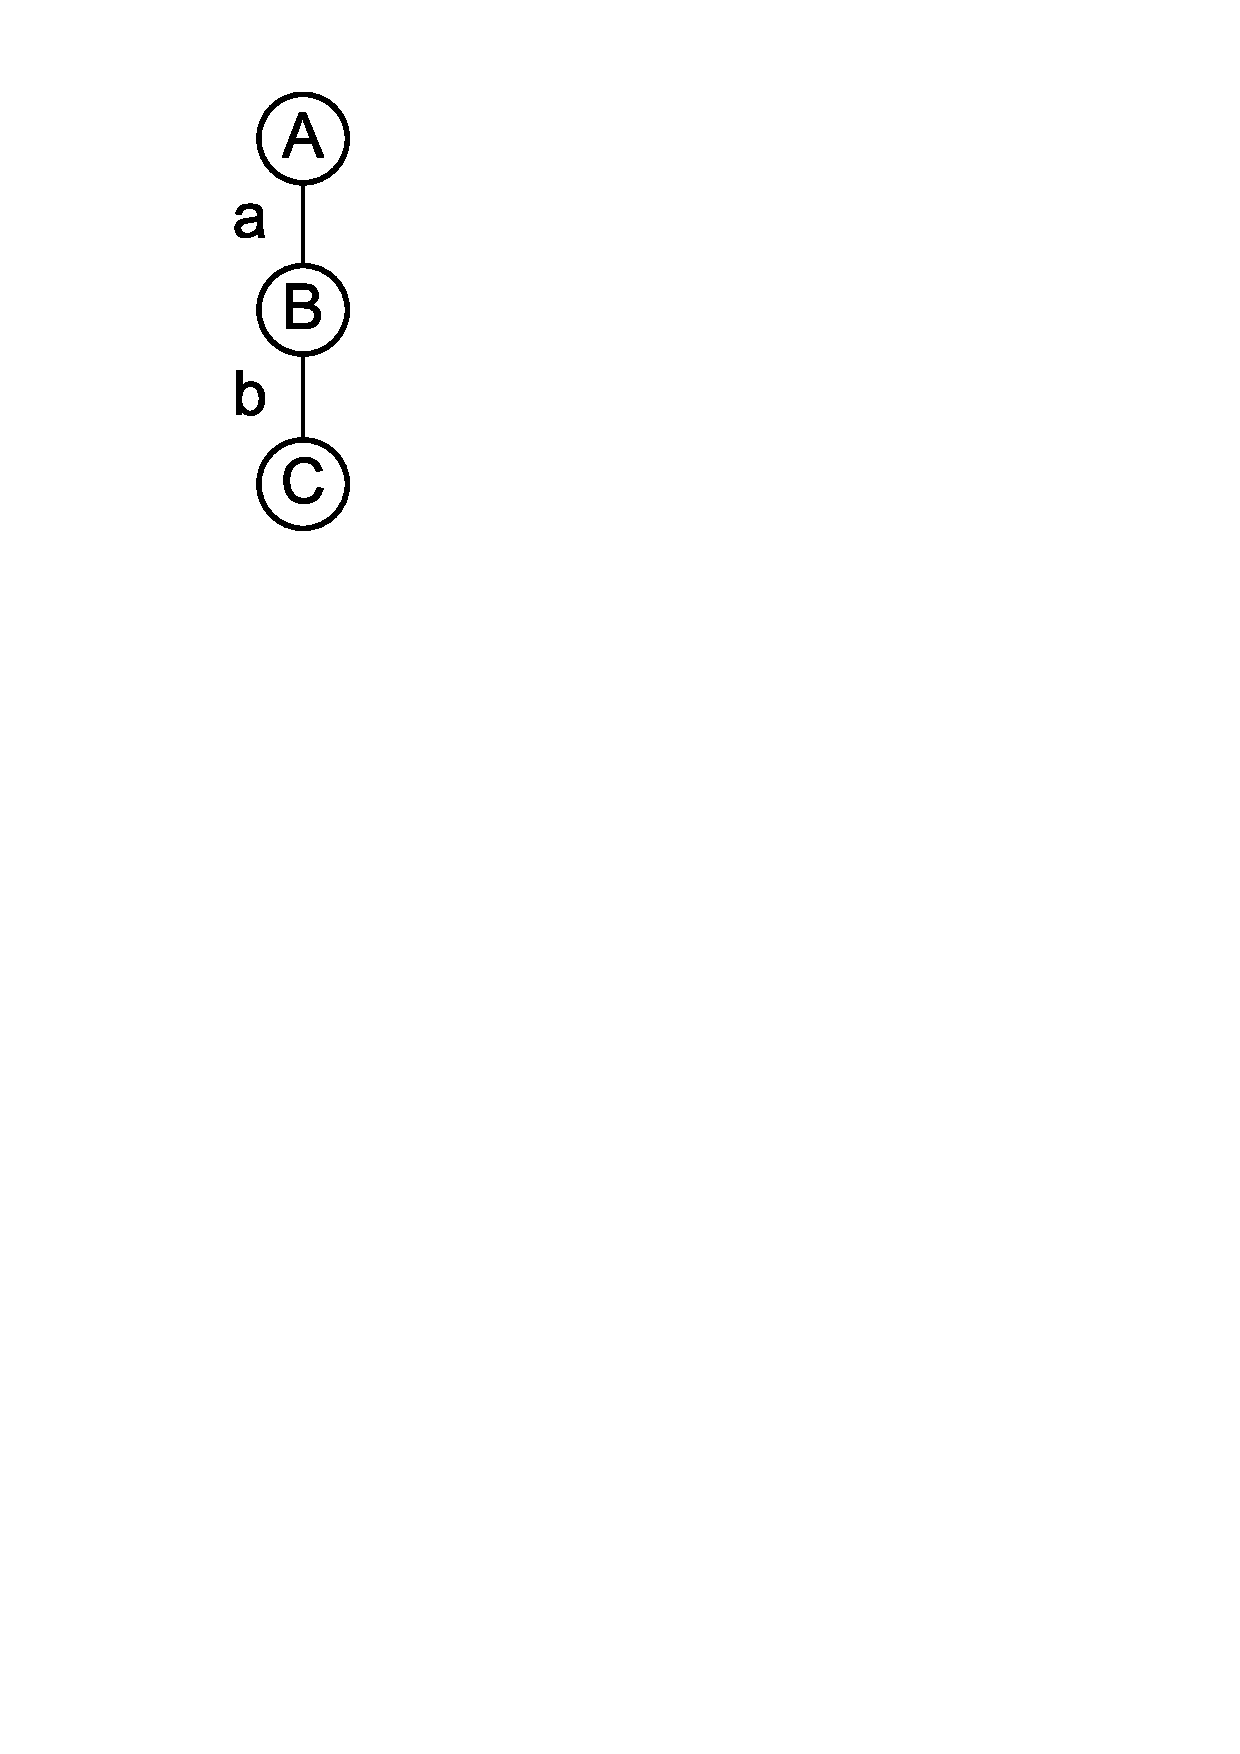
\includegraphics[scale=0.33]{images/replica1}
\label{fig:replica1}
}
\subfigure[{\scriptsize Occurrence of $Q$}]  {
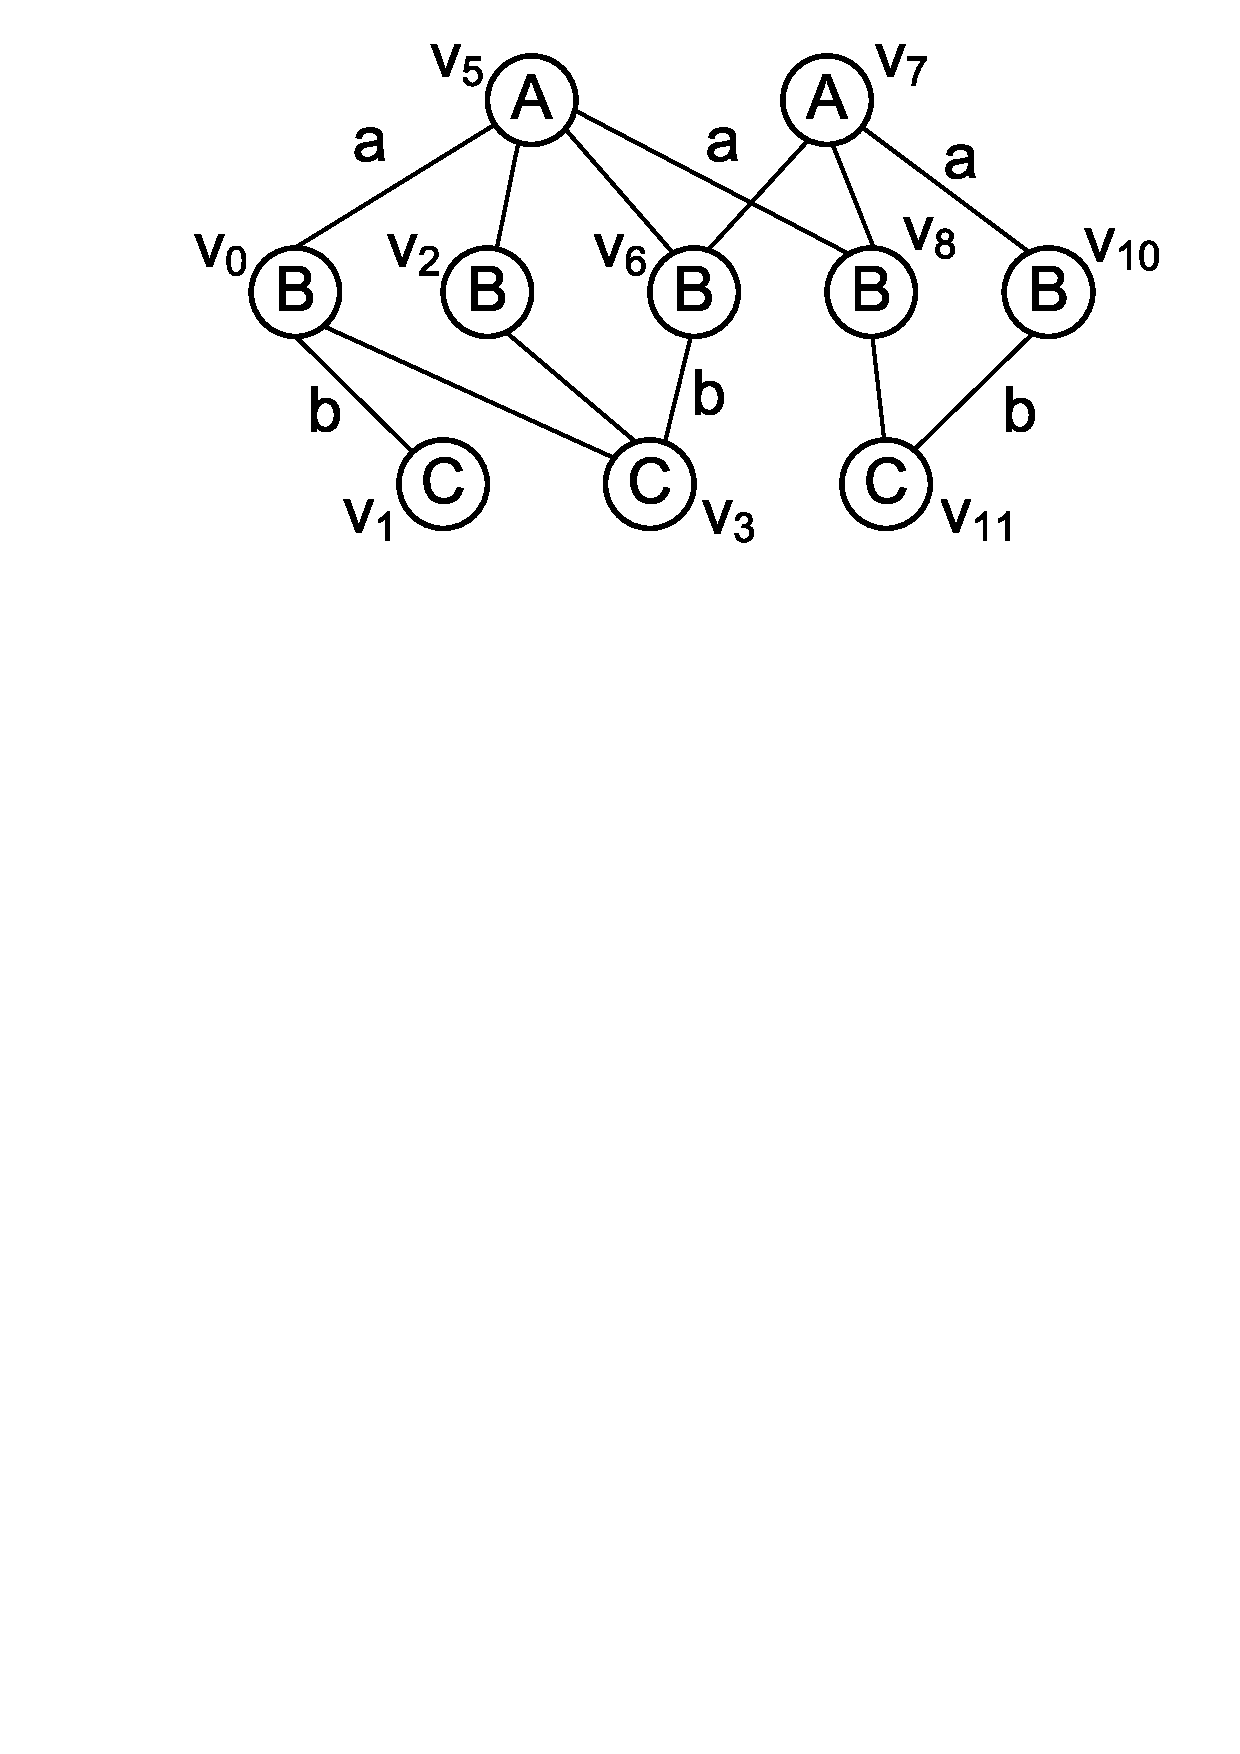
\includegraphics[scale=0.30]{images/replica2}
\label{fig:replica2}
}
\subfigure[{\scriptsize Replica of $Q$}]  {
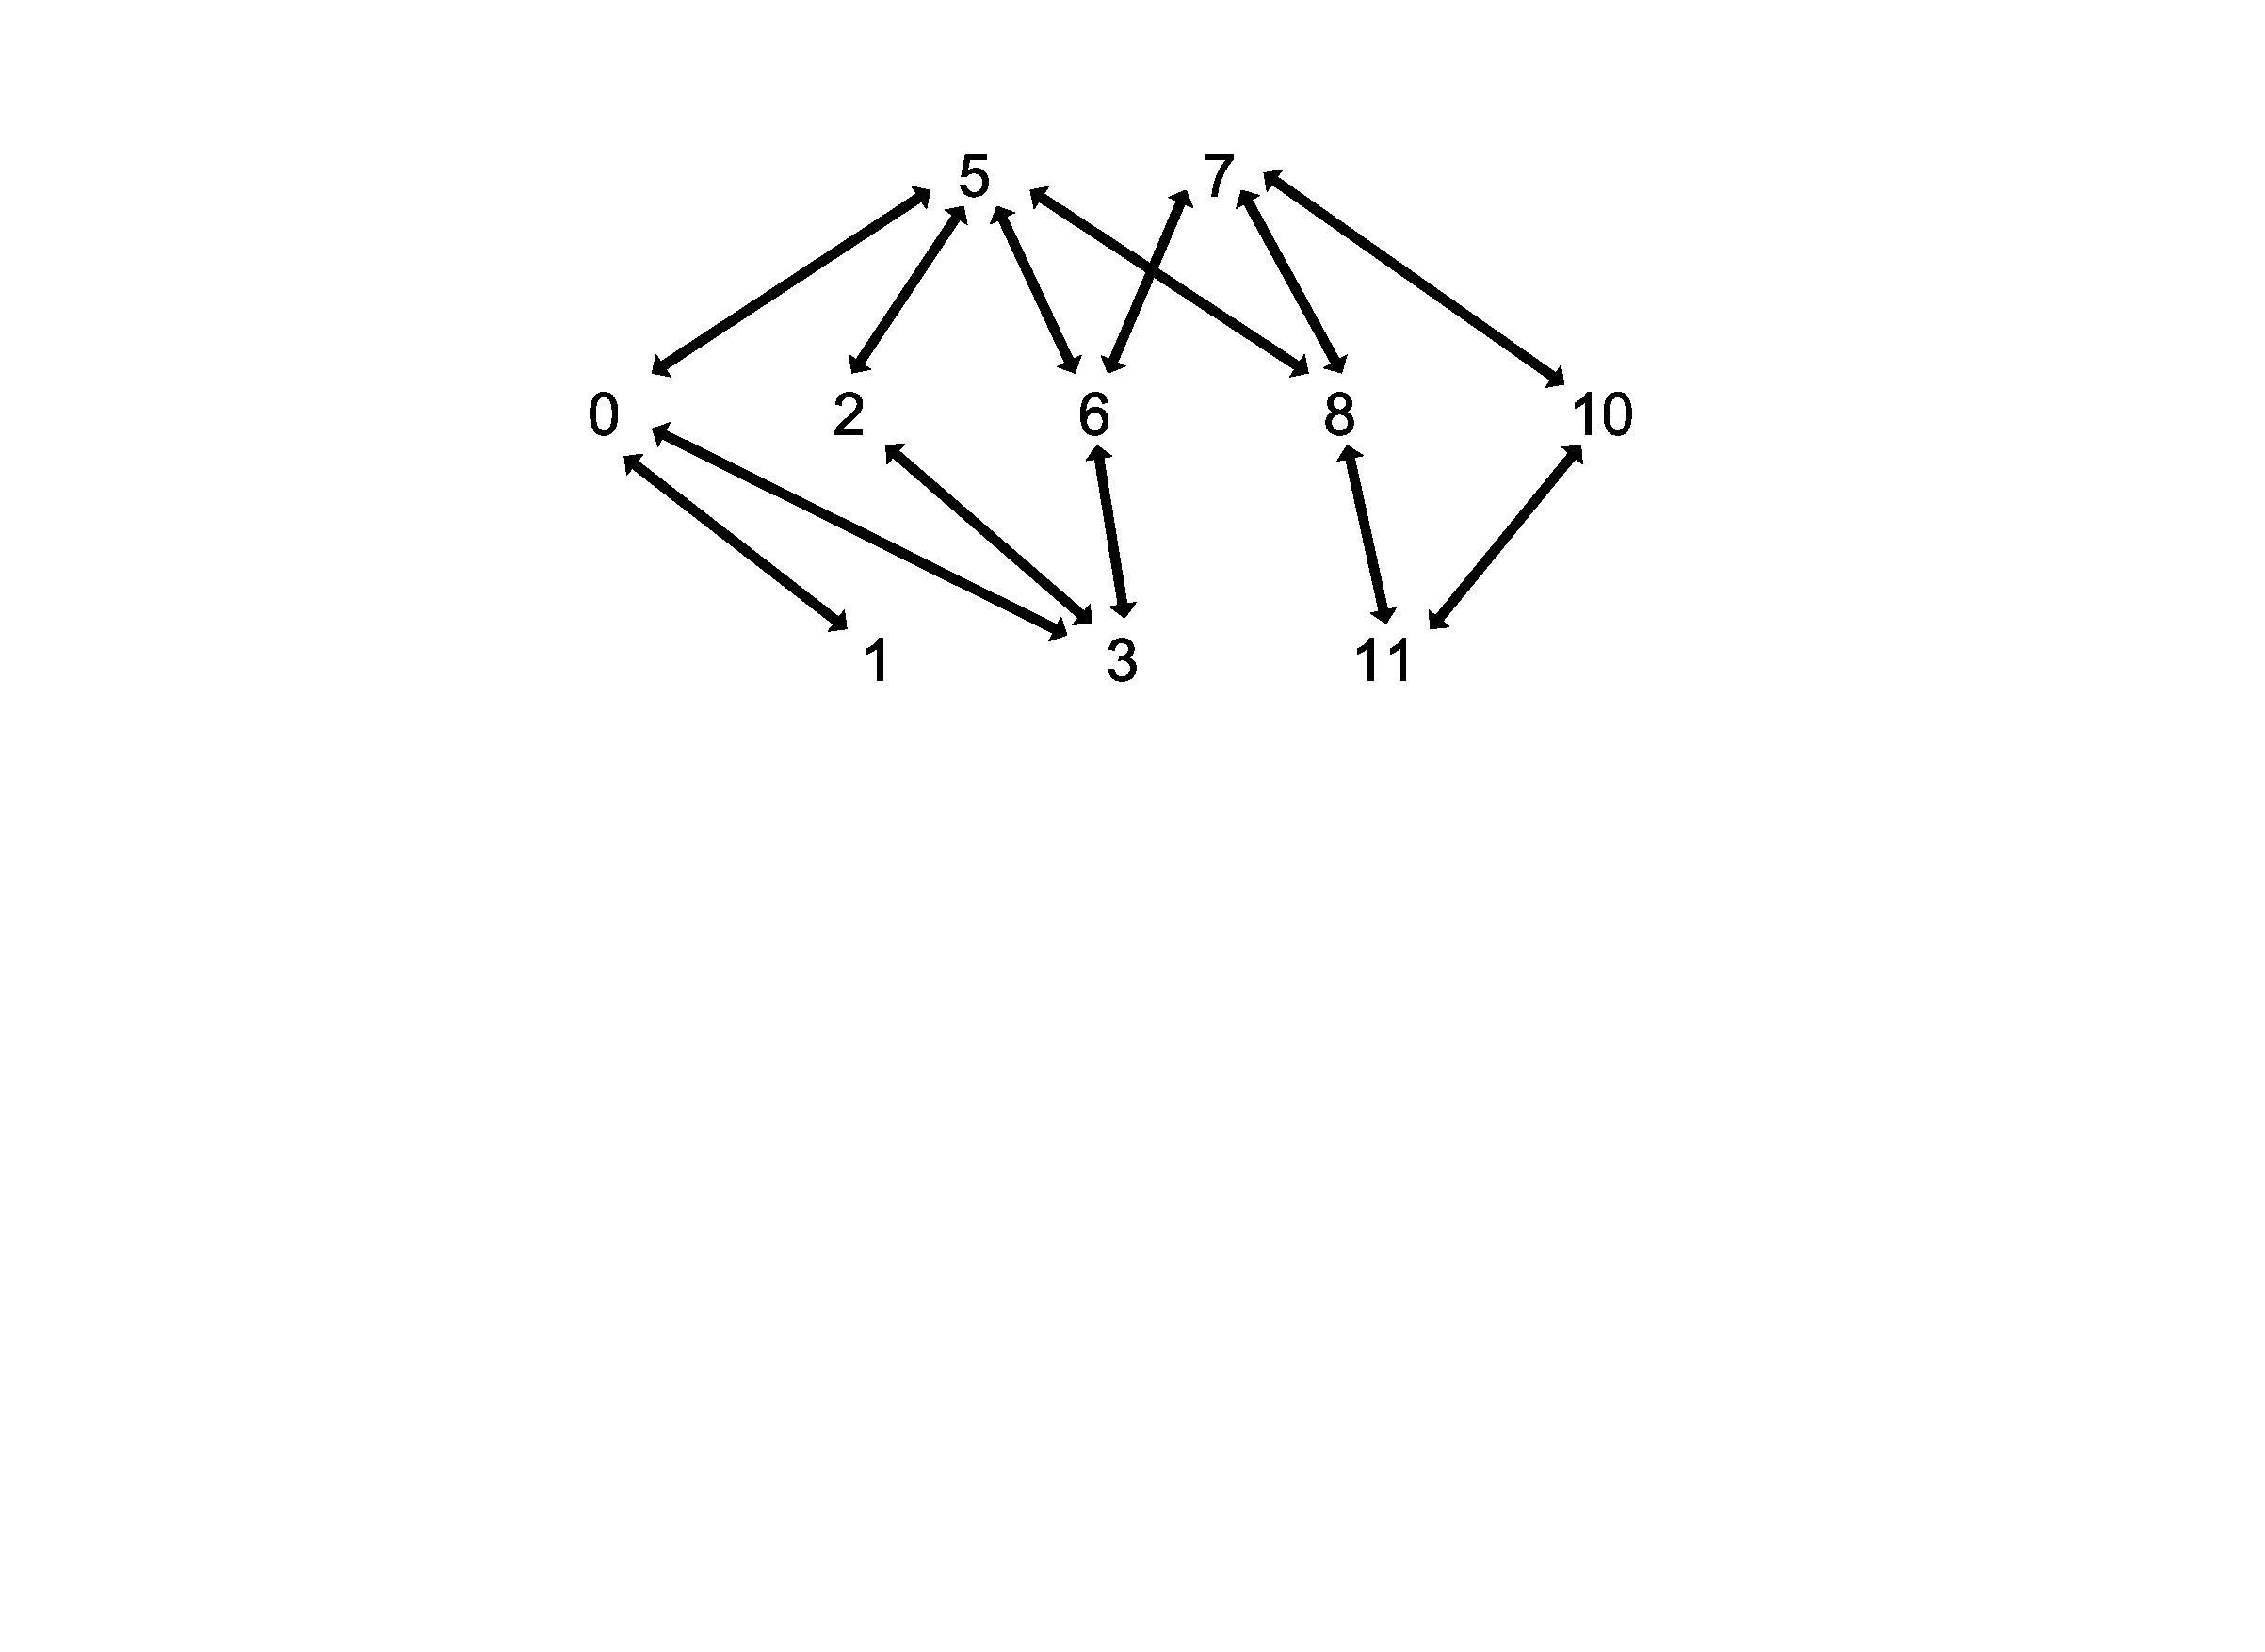
\includegraphics[scale=0.25]{images/replica3}
\label{fig:replica3}
}
\vspace{-2mm}
\caption{\scriptsize All the edge in Figure \ref{fig:replica2} from $A$ to $B$, $B$ to $C$ has the edge label $a,b$ respectively. Figure \ref{fig:replica3} is replicated from Figure \ref{fig:replica2} without edge labels.}
\label{fig:replica}
\vspace{-6mm}
\end{figure}
\newline
\newline
% As {\sf Found($Q$)} occurs, we store the replica of $Q$ as a unit of the search tree. 
After $Q$ has been $operated$, we remove $replica(Q)$ from memory.

\spara{$\bullet$ Replica Unit.} The illustration of replica is as Figure \ref{fig:replica}. The details of replica is as follows.\\1) For each $Q\in T$, there is a corresponding replica $R(Q)$.\\2) For each $u_i\in Q$, there is a hash-map, $R_i(Q)$, recording the vertex identifications, and $R(Q)=(R_1(Q), R_2(Q), ..., R_{|V_Q|}(Q))$.\\3) For each element $v\in R_i(Q)$, there is a record of all the other vertices which $v$ is connected to in the occurrences of $Q$.

Algorithms 1 and 2 together describe the complete procedure to construct the replica graph for a subgraph pattern. Replica construction for any pattern $R$ requires knowledge of the replica graph of the pattern $Q$ that is extended to generate it. Henceforth, we refer to such a pattern $R$ as a $child\ pattern$ of $Q$ and $Q$ as the $parent\ pattern$ of $R$. Since the search procedure processes a pattern only after its parent, the replica graph of the $parent\ pattern$ can be used for constructing the replica graph of the $child\ pattern$.  

    \begin{algorithm}
	\caption{Get Replica}\label{algo:search}
	\begin{algorithmic}[1] 
	\REQUIRE input graph: $G$, parent pattern: $Q$, replica of $Q$: $replica(Q)$, extending index: $u$, tuple of extension vertex label and extension edge label: $candidate\ edge$, child pattern: $R$
	\ENSURE all mappings of child pattern $R$ in $G$ (that is, the replica of $R$: $replica(R)$ in $G$)
	\STATE $DFS\ List\leftarrow$ get rooted {\sf DFS} of $Q$ with $u$ as $root$
	\FOR{\textbf{each} $m \in Mappings(u)$ in $replica(Q)$}
	\FORALL{adjacent edges $edge$ of $m$ that map to $candidate\ edge$}
    \STATE initialize set $instance$ with $edge$
	\STATE $\mathbb{I}\leftarrow$ {\sf find\ all\ instances($R$, $edge$, $instance$, $DFS\ List$)}
    \STATE Append all edges in $\mathbb{I}$ to $replica(R)$ and update the mappings list for every vertex
% 	\STATE $replica(R)\leftarrow replica(R) \cup \mathbb{I}$ 
% 	\IF{$instances\ set$ $\mathbb{I}$ is \textbf{not} empty}
% 	\STATE $replica(R)\leftarrow replica(R) \cup edge$ 
% 	\ENDIF
	\ENDFOR
	\ENDFOR
	\end{algorithmic}
	\end{algorithm}

Algorithm 1 essentially describes a procedure to find every mapping (also referred to as $instance$) of the $child\ pattern$ in the input graph using the mappings of the $parent\ pattern$ and thus obtain its $replica$ graph. The algorithm begins with a depth-first search ({\sf DFS}) procedure (line 1) executed on the $parent\ pattern\ Q$, selecting the vertex from which the $candidate\ edge$ is extended as the $root$. We call this vertex the $extending\ vertex$ in $Q$. The edges encountered in the depth-first traversal are recorded in an ordered list called the $DFS\ List$, which helps guide the instance enumeration procedure performed subsequently. The algorithm iterates over all mappings of the $extending\ index$ in the $replica$ of the $parent\ pattern$ (line 2) and attempts to enumerate all (if any) instances of the $child\ pattern$ in the input graph one-by-one. More specifically, for every vertex $m$ of $replica(Q)$ that maps to the $extending\ vertex\ u$, the algorithm iterates over its adjacent edges in the input graph that map to the $candidate\ edge$ (line 3) and invokes the {\sf find\ all\ instances} method (Algorithm 2) to enumerate every $instance$ of $child\ pattern\ R$ from $replica(Q)$ that contains this adjacent edge. Algorithm 2, thus invoked, recursively enumerates all instances of $R$ in a depth-first manner following the $DFS\ List$ of $Q$ (computed earlier). In the general case (lines 4-10), the algorithm selects an appropriate graph edge as the mapping of an edge in the $child\ pattern\ R$ (line 5) and recursively invokes the method to find a mapping of the next edge in the $DFS\ List$ that is consistent with the edge mappings selected so far (line 7). Once all edges in the $DFS\ List$ have been mapped to graph edges, the base case (lines 1-3) gets executed where the instance of $R$ thus enumerated is simply returned. Thus, the set of all instances found is returned at the end of Algorithm 2 (line 10) and recorded by Algorithm 1 to update the $replica$ graph (line 6, Algorithm 1). In the update step, the algorithm simply appends all edges of every instance in $\mathbb{I}$ to the existing set of edges of $replica(R)$, and also updates the $mappings\ set$ for every vertex of pattern $R$ to include the vertices of the newly-discovered instances in $\mathbb{I}$. 
% The {\sf find all instances()} function used in Algorithm ? is defined below. It enumerates all instances in a depth-first manner starting from the $extending\ index$ as the $root$ by following the {\sf DFS} edge-ordering stored in $DFS\ List$.
    \begin{algorithm}
	\caption{find all instances (complete)}\label{algo:complete-instances}
	\begin{algorithmic}[1] 
	\REQUIRE input graph: $G$, parent pattern: $Q$, replica of $Q$: $replica(Q)$, parent edge: $(u, v)$, $DFS\ List$ of $Q$ rooted at $extending\ index$, child pattern: $R$
	\ENSURE all mappings of pattern $R$ in $G$ that include $(u, v)$ 
	\IF{all $edges$ in $DFS\ List$ have been mapped}
	\STATE \textbf{return} $instance$ set 
	\ENDIF
	\FORALL{adjacent edges $e$ of $v$ in $replica(Q)$}
	\IF{$e$ maps to the corresponding $child\ edge$ in $DFS\ List$ \textbf{and} \textbf{not} already in $instance$}
	\STATE $instance\leftarrow instance\cup e$
	\STATE $\mathbb{I}\leftarrow \mathbb{I}\ \cup\ ${\sf find\ all\ instances($R$, $e$, $instance$, $DFS\ List$)}
	\ENDIF
	\ENDFOR
	\STATE \textbf{return} $\mathbb{I}$
	\end{algorithmic}
	\end{algorithm}

This replica storage strategy not only builds a foundation for the sequential efficient correlation calculation, but also benefits the MNI support counting in the single large graph since we can directly get $\sigma(Q)$ when we record the replica of $Q$ just by counting all the sizes of the images $M(v)$, where $v\in Q$.

\subsection{Subgraph Extension}
\subsubsection{Extension Rule}
We subscript the node patterns in a subgraph patterns to identify their order of discovery.
\begin{defn}[Vertices Subscripting]
	Let $Q$ be a frequent subgraph in $T$, apart from vertex identification $v_i$, we use another metric to subscript the vertices in $Q$ by the order we discover the pattern $Q$, denoted as $S_Q=(s_0,s_1,...,s_n)$, where $n=|V_Q|$. And for $s_i$ and $s_j$, if $i<j$, then the vertex $v_i$ is discovered earlier than the vertex $v_j$.
\end{defn}	
Taking advantage of subscripting, it is easy to get the right-most path of a subgraph. Then, we only grow the new vertices in right-most path. Corresponding to the best-first-search strategy, the node with highest MNI support will be chosen, suppose $Q$. Then, for all the vertices in its right-most path of the replica of $Q$, we try one edge extension from them respectively, see Algorithm \ref{algo:extension}.
\begin{algorithm}
	\caption{Subgraph Extension}\label{algo:extension}
	\begin{algorithmic}[1] 
	\REQUIRE data graph $G$, subgraph pattern $Q$, replica of $Q$, {\sf Min-sup}
	\ENSURE frequent pattern set extended from $Q$, $Ex(Q)$
	\STATE $Ex(Q)\leftarrow\emptyset$
	\STATE $Rmpath\leftarrow$ right-most path of $Q$	
	\FORALL{$s$ in $Rmpath$}
	\STATE $Ex(Q)\leftarrow Ex(Q)\cup$ possible extensions
	\ENDFOR 	
	\FORALL{$ex$ in $Ex(Q)$}
	\IF{$\sigma(ex)<$ {\sf Min-sup}}
	\STATE $Ex(Q)\leftarrow Ex(Q)\setminus ex$
	\ENDIF
	\ENDFOR
	\RETURN $Ex(Q)$
	\end{algorithmic}
	\end{algorithm}

\subsubsection{Duplicated Subgraph Prunning}
To avoid the duplicated subgraph judgement, we take the advantage of the DFS code, and the minimum DFS code in gSpan\cite{YH02}, whenever a subgraph is founded, we get its DFS code, denoted as $C(Q)$ and remodel this subgraph by using this code. Then, we build the minimum DFS code of this subgraph $Q$. This minimum DFS code, denoted as $Z(Q)$ is the canonical label of this subgraph in our definition.

\par We use a dictionary $\mathbb{D}$ to store all the minimum DFS code we have discovered so far. When a subgraph $Q$ is discovered and its graph code $C(Q)$ has been transformed to minimum DFS code $Z(Q)$, we search $Z(Q)$ in the dictionary. If $Z(Q)\in \mathbb{D}$, then $Q$ must have been discovered before, so we prune $Q$.

% \par We carry out a Trie structure to realize the dictionary and record $index(Q)$ in the search tree in $\mathbb{D}$. The function of the recording the index would be specified in Section \ref{subsec:avoiding}.

